\section{Segmentando el núcleo en dos etapas}

El primer paso hacia la segmentación del núcleo en las cinco etapas marcadas como objetivo del trabajo consistió en segmentarlo primeramente en dos, aislando la fase de \textit{fetch} respecto de las unidades funcionales implicadas en el resto de etapas.

Esta división no conlleva la aparición de riesgos de datos puesto que tanto la escritura como la lectura de estos forman parte de la misma fase dentro del ciclo de procesamiento de las instrucciones. Sin embargo, esta segmentación sí da pie a que, durante la ejecución de un programa, puedan aparecer riesgos de control tal y como se muestra en el ejemplo presentado en la Figura 5.6, donde la ausencia de mecanismos que logren mitigar el riesgo de control provoca la lectura de la instrucción señalada en color rojo antes de que se haya evaluado siquiera la condición en la instrucción de salto, ejecutando así la instrucción de resta y depositando en el registro \texttt{x1} un valor incoherente con la lógica del programa.

\begin{figure}[h]
  \centering
  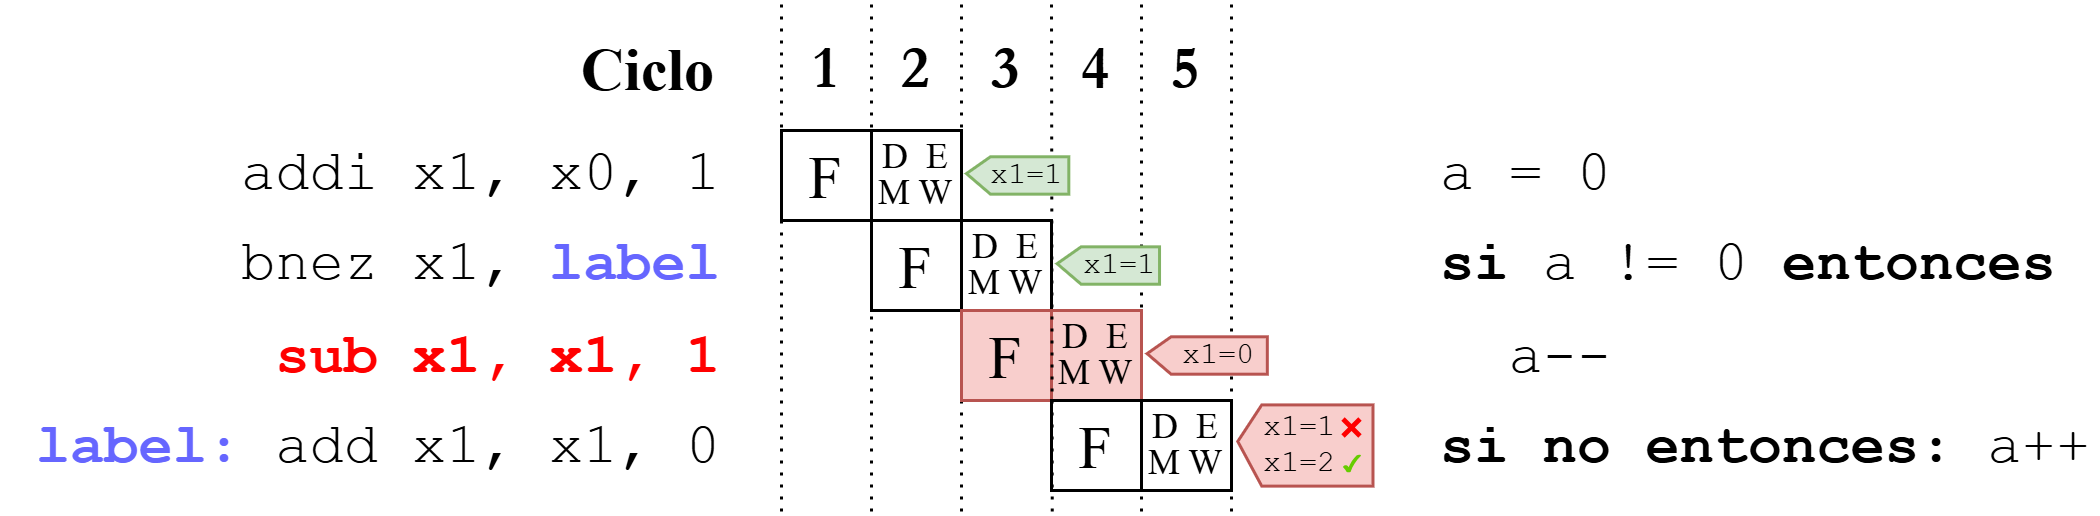
\includegraphics[width=0.9\linewidth]{res/img/diagramas/cap05_2_problema2etapas/cap05_2_problema2etapas.png}
  \vspace{+0.05cm}
  \caption{Representación del flujo de ejecución de un programa sobre una arquitectura segmentada en dos etapas sin mecanismos para resolver riesgos de control.}
\end{figure}

Para verificar la existencia o no del riesgo de control tras la introducción en la arquitectura del primer registro de segmentación, se desarrolló un sencillo programa en lenguaje ensamblador el cual incorpora instrucciones de salto condicional, salto incondicional y una llamada a función. Este programa (cuyo código se muestra en la Figura 5.7) fue compilado, cargado en memoria y ejecutado en el computador simulado por medio del test de Chisel mostrado en la Figura 5.8. El test consta, en primer lugar, de un bucle de inicialización en el que se espera a que el cargador lea el contenido del binario y lo deposite en la memoria del computador. Posteriormente, se ejecuta un segundo bucle en el que se hace avanzar el reloj 100 ciclos, a priori, suficientes como para recoger la ejecución completa del programa en la traza VCD resultante de la ejecución del test.

El primero de los problemas que se observó al examinar la traza generada por el test fue la falta de sincronismo entre el valor del contador de programa observado en una etapa determinada, y la instrucción observada en esa misma etapa, tal y como aparece señalado en color rojo en la Figura 5.9. En esa sección de la traza se muestran los cambios en el valor de las siguientes señales:

\begin{itemize}
  \item{\textbf{instr\_addr@fetch}: la dirección de la instrucción presente en la fase de fetch.}
  \vspace{-0.2cm}
  \item{\textbf{instr\_addr@DEMW}: la dirección de la instrucción en la fase siguiente al fetch.}
  \vspace{-0.2cm}
  \item{\textbf{instr@fetch}: la instrucción leída en la última fase de fetch.}
  \vspace{-0.2cm}
  \item{\textbf{instr@DEMW}: la instrucción leída en el anterior fetch.}
  \vspace{-0.2cm}
  \item{\textbf{fetch\_io\_jump\_flag}: la señal que indica si la evaluación de una condición es positiva y debe leerse por tanto en el siguiente ciclo, no la instrucción siguiente al contador de programa actual, si no el \textit{target} del salto. Tanto el target como esta señal se originan en la fase siguiente al fetch, como parte de la fase de ejecución (módulo \textit{Execute}).}
  \vspace{-0.2cm}
  \item{\textbf{ex\_io\_immediate}: el offset empleado en el cálculo de la dirección efectiva de salto, también como parte de la fase de ejecución.}
  \vspace{-0.2cm}
  \item{\textbf{ex\_io\_instr\_addr}: la dirección base del salto.}
  \vspace{-0.2cm}
  \item{\textbf{fetch\_io\_jump\_addr}: la dirección efectiva del salto. Esta señal llega al módulo \textit{InstructionFetch} desde \textbf{Execute}.}
\end{itemize}

% NOTE: Figura 5.7: Desensamblado, código ensamblador y pseudocódigo del programa empleado en la depuración de la arquitectura
\begin{figure}[h!]
\centering
\renewcommand{\arraystretch}{1}

\begin{tabular}{|p{0.30\textwidth}|p{0.30\textwidth}|p{0.30\textwidth}|}
\hline

\textbf{Código máquina} &
\textbf{Ensamblador} &
\textbf{Pseudocódigo} \\
\hline

\begin{lstlisting}[style=RiscVStyle]
  00000000 <_start>:
    0:  00000313
    4:  00400393

  00000008 <loop_start>:
    8:  0063ca63
    c:  00030513
    10: 010000ef
    14: 00050313
    18: ff1ff06f

  0000001c <loop_end>:
    1c: 0000006f
    
  00000020 <suma_uno>:
    20: 00050293
    24: 00128293
    28: 00028513
    2c: 00008067
\end{lstlisting}

&

\begin{lstlisting}[style=RiscVStyle]
  
  li    t1,0
  li    t2,4


  blt   t2,t1,loop_end
  mv    a0,t1
  jal   suma_uno
  mv    t1,a0
  j     loop_start


  j     loop_end


  mv    t0,a0
  addi  t0,t0,1
  mv    a0,t0
  ret
\end{lstlisting}

&

\begin{lstlisting}[style=RiscVStyle]
  
  t1 = 0
  t2 = 4
  
  
  mientras t1 < t2
  
    t1 = suma_uno(t1)
  



  
  
  función suma_uno(x)
    retornar x + 1
  
\end{lstlisting}

\\
\hline
\end{tabular}

\caption{Desensamblado, código ensamblador y pseudocódigo del programa empleado en la depuración de la arquitectura.}
\end{figure}

\vspace{1cm}

% NOTE: Figura 5.8: Código del test con el que se pone a prueba el funcionamiento de un programa sencillo sobre el núcleo segmentado en dos fases
\begin{figure}[h!]
\begin{lstlisting}[style=scalaStyle,columns=fullflexible]{}
class SegRegFDTest extends AnyFlatSpec with ChiselScalatestTester {
  behavior.of("Pipelined CPU")
  it should "run a simple program" in {
    test(new TestTopModule("simple_subroutine.asmbin"))
      .withAnnotations(TestAnnotations.annos) { c =>
      while(!c.io.instruction_valid.peek().litToBoolean) {
        c.clock.step()
        c.io.mem_debug_read_address.poke(4.U)
      }
      
      for (i <- 1 to 100) {
        c.clock.step()
        c.io.mem_debug_read_address.poke((i * 4).U)
      }

      c.io.regs_debug_read_address.poke(6.U)  // x6 => t1
      c.io.regs_debug_read_data.expect(5.U)
    }
  }
}
\end{lstlisting}
\vspace{-0.4cm}
\caption{Código del test con el que se pone a prueba el funcionamiento de un programa sencillo sobre el núcleo segmentado en dos fases.}
\end{figure}

\vspace{+0.2cm}

La consecuencia que esta falta de sincronismo tiene sobre el flujo de ejecución de los programas es que las instrucciones de salto no pueden realizar correctamente el cómputo de la dirección efectiva de este, al contar en la fase de ejecución con el contador de programa de la instrucción siguiente al salto, y no la del propio salto. Tal y como se observa en la traza de la Figura 5.9, al comienzo del ciclo marcado en la posición en que se encuentra el indicador vertical (43 ps), la instrucción \texttt{jal suma\_uno} (\texttt{0x010000EF @ 0x1010\footnote{El punto de entrada de los programas se encuentra en la dirección \texttt{0x1000}. La dirección de la instrucción es el valor del punto de entrada sumado al offset mostrado en la primera columna de la Figura 5.7}}, ver señal \texttt{instr@DEMW}), observa los siguientes operandos en el cálculo del destino del salto:

\begin{itemize}
  \item{\textbf{ex\_io\_immediate}: \texttt{0x10}}
  \vspace{-0.2cm}
  \item{\textbf{instr\_addr@DEMW}: \texttt{0x1014}}
\end{itemize}

Puede observarse que la dirección base del salto no es la correspondiente a la instrucción \texttt{jal}, si no la de la instrucción \texttt{mv} que la sucede en el programa, provocando que el salto no sea al comienzo de la subrutina \texttt{suma\_uno}, si no a la segunda instrucción dentro de esta.

\vspace{+0.2cm}

% NOTE: Figura 5.9: Seccion de la traza obtenida tras la ejecucion del test mostrado en la Figura 5.7
\begin{figure}[h]
  \centering
  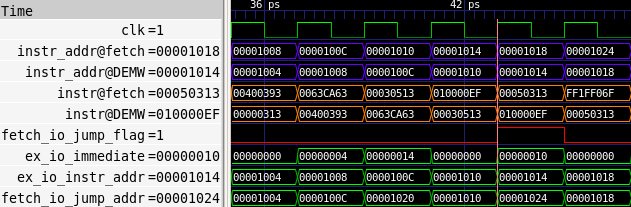
\includegraphics[width=0.67\linewidth]{res/img/diagramas/cap05trazaGTKwaveNoCheck/cap05trazaGTKwaveNoCheck.png}
  \caption{Sección de la traza obtenida tras la ejecución del test mostrado en la Figura 5.7}
\end{figure}

\vspace{+0.2cm}
% TODO: añadir referencia a https://www.chisel-lang.org/docs/explanations/memories
El diseño original emplea como memoria una instancia de la clase \textit{SyncReadMem}. Este tipo de memoria no permite realizar lecturas de manera asíncrona, lo cual implica que, cuando se solicita una lectura, el dato leído no sale de la memoria hasta el siguiente flanco ascendente de reloj, impidiendo que se mantenga la sincronía entre las instrucciones en cada fase y la dirección de la instrucción observada en esa misma fase. En el computador objeto de este trabajo, este comportamiento de la memoria se materializa en que, cuando se envía la dirección de una instrucción para leerla, esa lectura no será efectiva hasta el ciclo siguiente al envío de la dirección. De ahí que, por ejemplo, la dirección de una instrucción en la fase de fetch (señal \texttt{instr\_addr@fetch}) no se corresponda con la instrucción observada en esa misma fase (señal \texttt{instr@fetch}), si no con la instrucción inmediatamente anterior a la solicitada.

Para solucionar esta problemática se cambia, dentro de la clase \textit{Memory}, el tipo de memoria a una de la clase \textit{Mem}, de forma que la lectura del dato se lleve a cabo en el instante mismo en que se solicita. De este modo, tal y como puede observarse en la traza presentada en la Figura 5.10, el valor de la dirección de la instrucción en cada fase se corresponde con la de la instrucción que se está procesando en esa misma fase, de tal modo que ahora el cálculo del \textit{target} en la instrucción de salto sea correcto (\texttt{0x1010} (\texttt{ex\_io\_instr\_addr}
) + \texttt{0x10} (\texttt{ex\_io\_immediate}) = \texttt{0x1020} (\texttt{fetch\_io\_jump\_addr}) $\rightarrow$ \texttt{suma\_uno}).

% NOTE: Figura 5.10: Misma seccion de la traza pero con una instancia de la clase Mem como entidad de memoria en lugar de SyncReadMem.
\vspace{+0.2cm}
\begin{figure}[h]
  \centering
  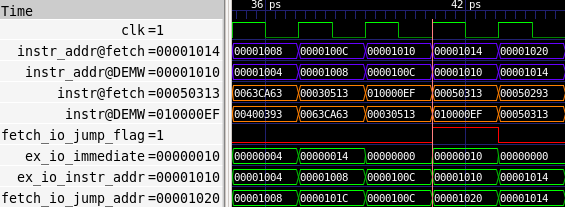
\includegraphics[width=0.65\linewidth]{res/img/diagramas/cap05trazaGTKwaveNoCheck/cap05trazaGTKwaveNoCheckAfterSyncReadMemChangeToMem.png}
  \caption{Misma sección de la traza pero con una instancia de la clase \texttt{Mem} como entidad de memoria en lugar de \texttt{SyncReadMem}.}
\end{figure}

\vspace{+0.2cm}

A pesar de esta corrección, puede observarse que el flujo de ejecución del programa sigue siendo erróneo ya que, siguiendo a la instrucción de salto (tras la marca vertical), en la segunda fase logra introducirse y ejecutarse la instrucción inmediatamente posterior, la cual es un \texttt{mv t1, a0} (\texttt{0x00050313 @ 0x1014}). En el caso concreto de la primera iteración del bucle, la ejecución de esta instrucción es inócua ya que en ese punto los registros \texttt{t1} y \texttt{a0} albergan el mismo valor. No obstante a esto, la inserción de la instrucción siguiente al salto toma una relevancia significativa cuando se trata de otra instrucción de salto, tal y como ocurre tras el salto incondicional al final del bucle. La ejecución de este segundo salto, el cual forma parte del bucle de final de programa, provoca que este llegue a término tras la primera iteración (véase Figura 5.9).

% NOTE: Figura 5.11: Seccion de la traza en la que se muestra la pronta ejecucion del bucle final
\vspace{+0.5cm}
\begin{figure}[h]
  \centering
  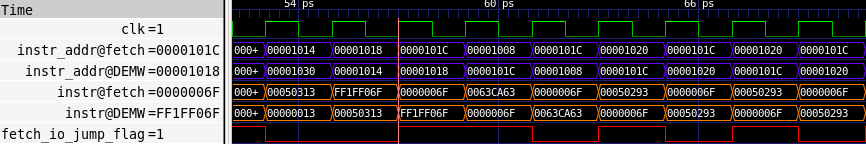
\includegraphics[width=\linewidth]{res/img/diagramas/cap05_syncreadmem_to_mem_end_loop/cap05_syncreadmem_to_mem_end_loop.png}
  \caption{Sección de la traza en la que se muestra la pronta ejecución del bucle final.}
\end{figure}
\vspace{+0.1cm}

La solución final para resolver esta problemática consiste en la introducción de un par de modificaciones en la fase de fetch para hacer que la arquitectura introduzca una operación \texttt{nop} tras cada instrucción de salto en cuya segunda fase se determine que este deba ser tomado. Estas modificaciones se realizan sobre la lógica que hace avanzar el contador de programa.

En la nueva implementación, tal y como se observa en el \texttt{diff} presentado en la Figura 5.12, se introduce un \texttt{nop} en el pipeline siempre y cuando se cumplan las dos condiciones siguientes: en primer lugar, que el cargador no haya terminado su trabajo y, en segundo lugar, que en la segunda fase de una instrucción de salto se haya determinado que este deba ser tomado (originalmente solo se contemplaba la primera condición).

% Figura 5.12: Comparación entre la implementación original del módulo \texttt{InstructionFetch} y su adaptación para resolver riesgos de control
\vspace{+0.2cm}
\begin{figure}[h]
\begin{lstlisting}[style=DiffStyleNoNumbering,columns=fullflexible]
   val pc = RegInit(ProgramCounter.EntryAddress)

-  when(io.instruction_valid) {
-    pc             := Mux(io.jump_flag_id, io.jump_address_id, pc + 4.U)
-    io.instruction := io.instruction_read_data
+  when(io.instruction_valid && !io.jump_flag_id) {
+    pc             := pc + 4.U
+    io.instruction := io.instruction_read_data
   }.otherwise {
-    pc             := pc
+    pc             := io.jump_address_id
     io.instruction := 0x00000013.U
   }

   io.instruction_address := pc
\end{lstlisting}
\vspace{-0.4cm}
\caption{Comparación entre la implementación original del módulo \texttt{InstructionFetch} y su adaptación para resolver riesgos de control.}
\end{figure}